\documentclass[11pt, oneside]{article}   	% use "amsart" instead of "article" for AMSLaTeX format
\usepackage{geometry}                		% See geometry.pdf to learn the layout options. There are lots.
\usepackage{enumitem}
\usepackage{mathtools}

\geometry{letterpaper}                   		% ... or a4paper or a5paper or ... 
%\geometry{landscape}                		% Activate for rotated page geometry
%\usepackage[parfill]{parskip}    		% Activate to begin paragraphs with an empty line rather than an indent
\usepackage{graphicx}				% Use pdf, png, jpg, or eps§ with pdflatex; use eps in DVI mode
								% TeX will automatically convert eps --> pdf in pdflatex		
\usepackage{amssymb}
\usepackage{multicol}

\usepackage{xcolor}
\usepackage{textcomp}
\usepackage{subfigure}

%SetFonts

%SetFonts
% code listing settings
\usepackage{listings}
\lstset{
    language=Python,
    basicstyle=\ttfamily\small,
    aboveskip={1.0\baselineskip},
    belowskip={1.0\baselineskip},
    columns=fixed,
    extendedchars=true,
    breaklines=true,
    tabsize=4,
    prebreak=\raisebox{0ex}[0ex][0ex]{\ensuremath{\hookleftarrow}},
    frame=lines,
    showtabs=false,
    showspaces=false,
    showstringspaces=false,
    keywordstyle=\color[rgb]{0.627,0.126,0.941},
    commentstyle=\color[rgb]{0.133,0.545,0.133},
    stringstyle=\color[rgb]{01,0,0},
    numbers=left,
    numberstyle=\small,
    stepnumber=1,
    numbersep=10pt,
    captionpos=t,
    escapeinside={\%*}{*)}
}


\title{Assignment 4}
\author{Omar Ghaleb\\
COMP 5107}
\date{}							% Activate to display a given date or no date

\begin{document}
\renewcommand\thesubsection{\alph{subsection}.}
\maketitle
%\section{}
%\subsection{}
%\begin{enumerate}[label=\alph*)]
%	\item First item
%\end{enumerate}
In this assignment we have two classes $X_1$ and $X_2$ with means same as the previous assignment $M_1$ and $M_2$ where: $$M_1 = \begin{bmatrix}
3 & 1 & 4 
\end{bmatrix},\quad M_2 = \begin{bmatrix}
-3 & 1 & -4 
\end{bmatrix}$$
  and covariance matrices as follows: 
  $$\sum_{X_1} = \begin{bmatrix}
a^2 & \beta ab & \alpha ac \\
\beta ab & b^2 & \beta bc \\
\alpha ac & \beta bc & c^2 
\end{bmatrix},\quad \sum_{X_2} = \begin{bmatrix}
c^2 & \alpha bc & \beta ac \\
\alpha bc & b^2 & \alpha ab \\
\beta ac & \alpha ab & a^2 
\end{bmatrix}$$

The parameters used in this assignment is as follows:
$$ a=2,\quad b=3,\quad c=4,\quad \alpha=0.1,\quad \beta=0.2,\quad \#points = 2000 $$
This resulted the covariance matrices to have the following values:
$$\sum_{X_1} = \begin{bmatrix}
4 & 1.2 & 0.8 \\
1.2 & 9 & 2.4 \\
0.8 & 2.4 & 16 
\end{bmatrix}, \quad \sum_{X_2} = \begin{bmatrix}
16 & 1.2 & 1.6 \\
1.2 & 9 & 0.6 \\
1.6 & 0.6 & 4 
\end{bmatrix}$$


\subsection{Create points for each distribution:}

Here we used the same exact methods for creating the points from the previous assignment.
And the plots of the points are available below.

\begin{lstlisting}[label={list:first},caption=Gaussian vector generation]
# create point matrices for the two classes X1 and X2
z1_matrix, x1_matrix = h.generate_point_matrix(v_x1, lambda_x1, m1, number_of_points)
z2_matrix, x2_matrix = h.generate_point_matrix(v_x2, lambda_x2, m2, number_of_points)

# PLOTTING #
# plot the first class as blue for (d1 - d2) domain and second class as red
h.plot_2d_graph(x1_matrix, x2_matrix, 1, 2, 'x1', 'x2', 'x1-x2')

# plot the first class as blue for (d1 - d3) domain and second class as red
h.plot_2d_graph(x1_matrix, x2_matrix, 1, 3, 'x1', 'x3', 'x1-x3')
\end{lstlisting}


\subsection{Compute the optimal Bayes discriminant function:}

For calculating the Bayes discriminant function we use the quadratic function form of the matrices using the following equation:
$$ X^TAX+B^TX+C \lessgtr 0 $$
Then setting one variable to 0 and solving for the other two which will result in a quadratic equation.
For $(x_1-x_2)$:
$$(a_{22})x_2^2+(a_{12}x_{1}+a_{21}x_{1}+b_{12})x_2+(a_{11}x_1^2+b_{11}x_1+c)=0$$
For $(x_1-x_3)$:
$$(a_{33})x_3^2+(a_{13}x_{1}+a_{31}x_{1}+b_{13})x_3+(a_{11}x_1^2+b_{11}x_1+c)=0$$


\begin{lstlisting} [label={list:first},caption=Simultaneous Diagonalization]
a = ((np.linalg.inv(sigma_x2) - np.linalg.inv(sigma_x1)) / 2)
b = np.array(m1.transpose() @ np.linalg.inv(sigma_x1) - m2.transpose() @ np.linalg.inv(sigma_x2))
c = np.math.log(p1 / p2) + np.log(np.linalg.det(sigma_x2) / np.linalg.det(sigma_x1))

equation_points = []
roots_1 = []
roots_2 = []

min_w = min(min(min(x1_matrix[0, :]), min(x2_matrix[0, :])),
            min(min(x1_matrix[1, :]), min(x2_matrix[1, :])))
max_w = max(max(max(x1_matrix[0, :]), max(x2_matrix[0, :])),
            max(max(x1_matrix[1, :]), max(x2_matrix[1, :])))

# get the roots for the discriminant function for (x1-x2)
for x1 in range(-15, 10, 1):
    equation_points.append(x1)
    x2_square_coefficient = a[1 	][1]
    x2_coefficient = (a[0][1] * x1) + (a[1][0] * x1) + b[0][1]
    constant = a[0][0] * np.math.pow(x1, 2) + b[0][0] * x1 + c

    poly_coefficients = [x2_square_coefficient, x2_coefficient, constant]
    roots = np.roots(poly_coefficients)
    roots_1.append(roots[0])
    roots_2.append(roots[1])

# get the roots for the discriminant function for (x1-x3) 
for x1 in range(-15, 15, 1):
    equation_points.append(x1)
    x2_square_coefficient = a[2][2]
    x2_coefficient = (a[0][2] * x1) + (a[2][0] * x1) + b[0][2]
    constant = a[0][0] * np.math.pow(x1, 2) + b[0][0] * x1 + c

    poly_coefficients = [x2_square_coefficient, x2_coefficient, constant]
    roots = np.roots(poly_coefficients)
    roots_1.append(roots[0])
    roots_2.append(roots[1])

\end{lstlisting}

\subsection{Generating 200 testing points and report the accuracy:}
Here we create 200 points in the $X$-world and try to classify them using the discriminant function that we calculated before.

If the $discriminant value > 0$, then class 1
and if $discriminant value < 0$, then class 2

\begin{lstlisting} [label={list:first},caption=Generating 5000 points]
+---------+---------+---------+----------+
|  Prd\Tr | class 1 | class 2 | Accuracy |
+---------+---------+---------+----------+
| class 1 |  180.0  |   20.0  |   90.0   |
| class 2 |   3.0   |  197.0  |   98.5   |
+---------+---------+---------+----------+
\end{lstlisting}

\subsection{Diagonalize the points:}
\begin{lstlisting} [label={list:first},caption=Generating 5000 points]
# diagonalizing the original points and the testing points
v1_matrix, v2_matrix, sigma_v1, sigma_v2, v1_mean, v2_mean = h.diagonalize_simultaneously(x1_matrix, x2_matrix, sigma_x1, sigma_x2, m1, m2)
v1_test_points, v2_test_points, _, _, _, _ = h.diagonalize_simultaneously(x1_test_points, x2_test_points, sigma_x1, sigma_x2, m1, m2)
\end{lstlisting}

\subsection{Computing the discriminant function for $V$-world:}
For this part i used the same method as part \textit{b}, but instead I used the covariance and means of the diagonalized points.

\subsection{Classify the same testing points in the $V$-world:}
We used the same exact 200 points here to test the new discriminant function that we created for the $V$-world. The values returned by the function were almost identical, they just differed in floating points which did not affect the classification accuracy. hence we got the results as follows:
\begin{lstlisting} [label={list:first},caption=Generating 5000 points]
After diagonalizing:
+---------+---------+---------+----------+
|  Prd\Tr | class 1 | class 2 | Accuracy |
+---------+---------+---------+----------+
| class 1 |  180.0  |   20.0  |   90.0   |
| class 2 |   3.0   |  197.0  |   98.5   |
+---------+---------+---------+----------+

\end{lstlisting}


\subsection{The graphs for the points and the discriminant function:}
The following graphs show the points generated in the $X$ world before diagonalization and also the calculated \textit{discriminant function}.
\newpage
%\begin{figure}
%\begin{center}
%	\subfigure[x1-x2]{
%	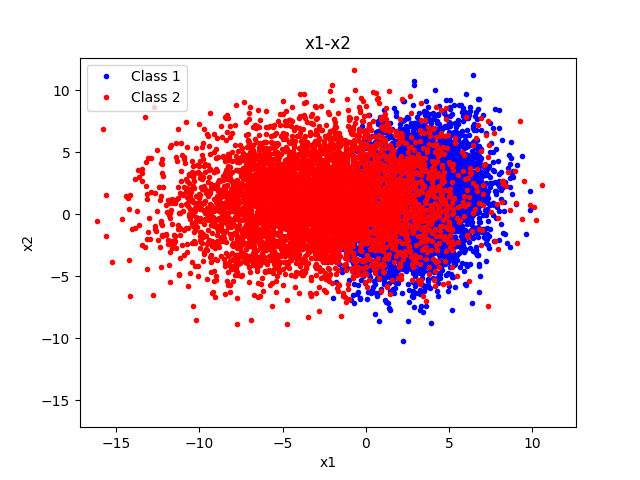
\includegraphics[width=0.45\textwidth]{x1-x2}
%	\label{absorbing}
%	}
%	\subfigure[x1-x2]{
%	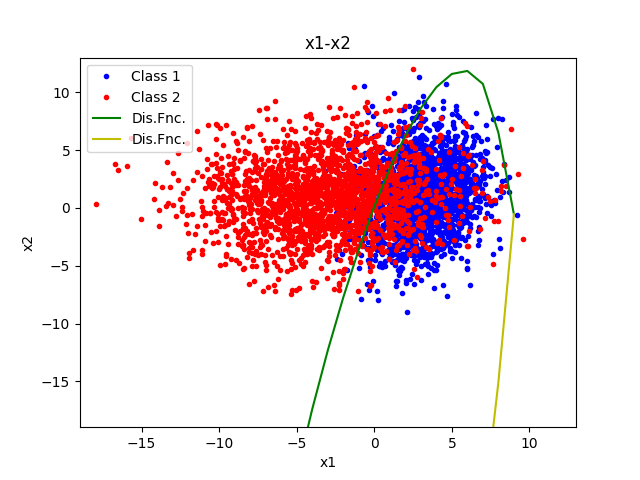
\includegraphics[width=0.45\textwidth]{x1-x2-disc-func}
%	\label{absorbing}
%	}\\
%	\subfigure[x1-x3]{
%	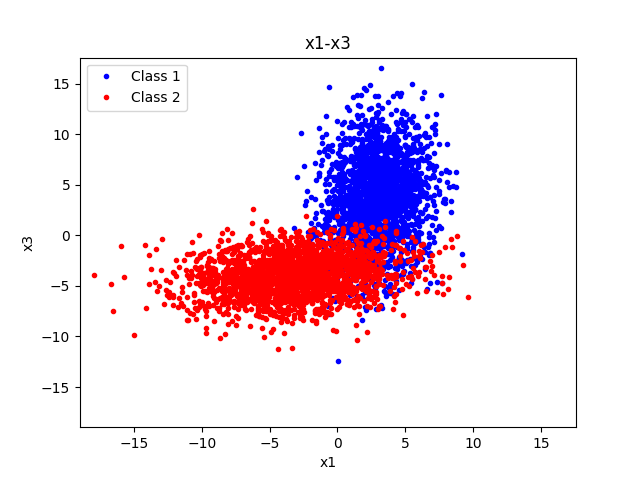
\includegraphics[width=0.45\textwidth]{x1-x3}
%	\label{absorbing}
%	}
%	\subfigure[x1-x3]{
%	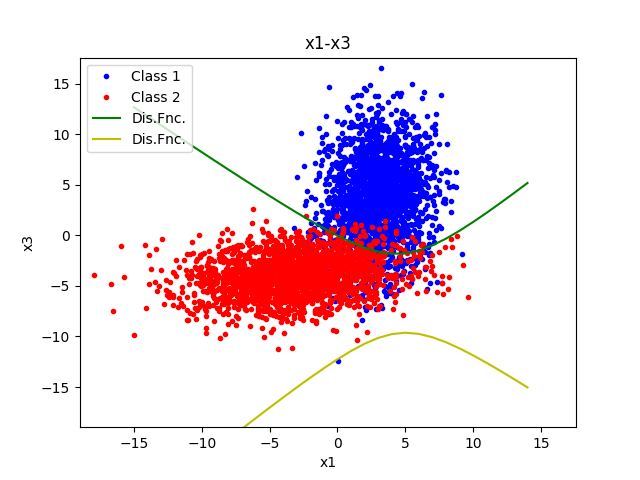
\includegraphics[width=0.45\textwidth]{x1-x3-disc-func}
%	\label{absorbing}
%	}
%\end{center}
%\caption{The generated points in $X$-world and the \textit{discriminant function}}
%\end{figure}
%
%\begin{figure}
%\begin{center}
%	\subfigure[v1-v2]{
%	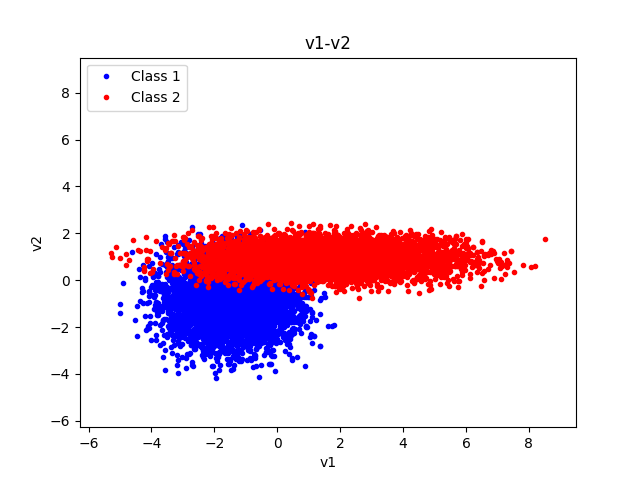
\includegraphics[width=0.45\textwidth]{v1-v2}
%	\label{absorbing}
%	}
%	\subfigure[v1-v2]{
%	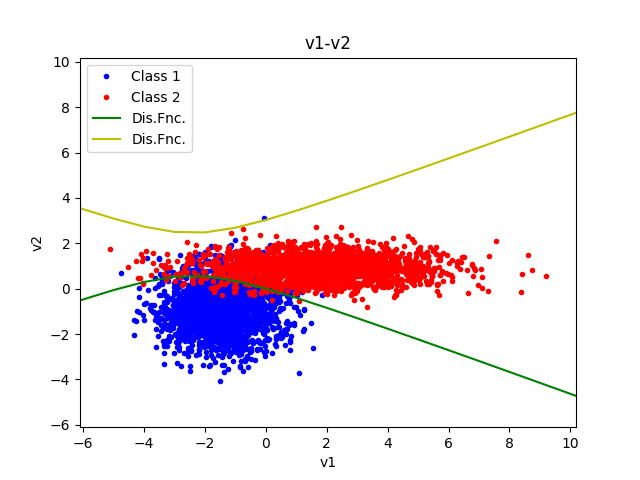
\includegraphics[width=0.45\textwidth]{v1-v2-disc-func}
%	\label{absorbing}
%	}\\
%	\subfigure[v1-v3]{
%	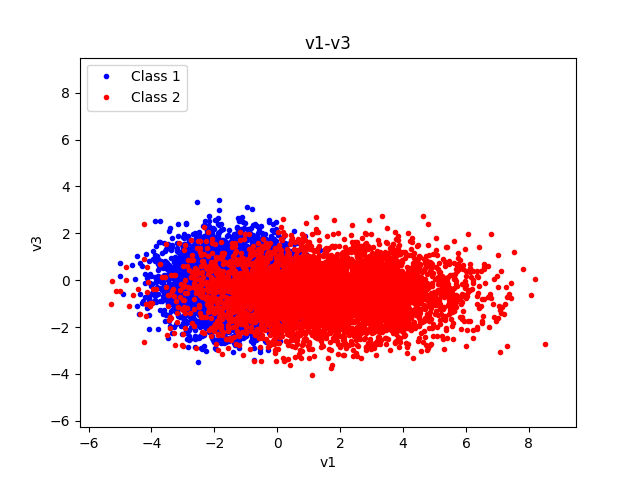
\includegraphics[width=0.45\textwidth]{v1-v3}
%	\label{absorbing}
%	}
%	\subfigure[v1-v3]{
%	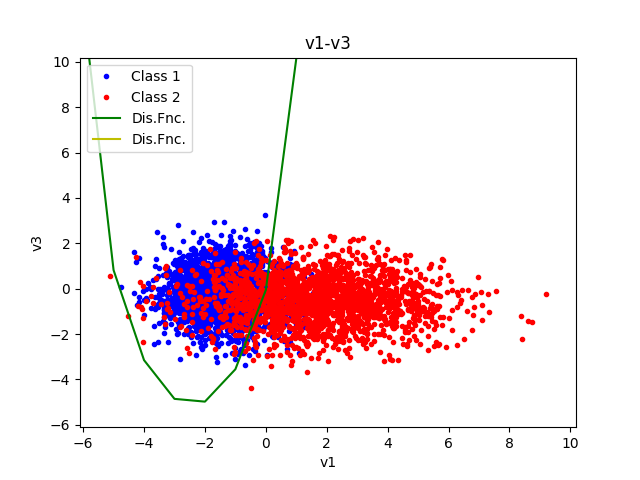
\includegraphics[width=0.45\textwidth]{v1-v3-disc-func}
%	\label{absorbing}
%	}
%\end{center}
%\caption{The generated points in $V$-world and the \textit{discriminant function}}
%\end{figure}




\end{document}  








